\section{Memory Management Hardware}

\paragraph{Main Memory}
\begin{itemize}
  \item main memory + registers = only storage that CPU can access directly
  \item \textbf{Before run}: program must be
  \begin{itemize}
    \item brought into memory from background storage
    \item placed within a process' address space
  \end{itemize}
  \item \textbf{Earlier}: computers had no memory abstraction
  \begin{itemize}
    \item[$ \to $] programs accessed physical memory directly
  \end{itemize}
  \item multiple processes can be run concurrently even without memory abstraction (using swapping, relocation)
\end{itemize}

\paragraph{Swapping}
\begin{itemize}
  \item \textbf{Principle}:
  \begin{itemize}
    \item \emph{roll-out}: save program's state on background storage
    \item \emph{roll-in}: replace program state with another program's state
  \end{itemize}
  \item \textbf{Advantages}:
  \begin{itemize}
    \item[+] only needs hardware support to protect kernel, not to protect processes from one another
  \end{itemize}
  \item \textbf{Disadvantages}:
  \begin{itemize}
    \item[-] \emph{very slow}: major part of swap time is transfer time
    \item[-] \emph{no parallelism}: only one process runs at a time, owns entire physical address space
  \end{itemize}
\end{itemize}

\paragraph{Overlays}
\begin{itemize}
  \item \textbf{Problem}: what if process needs more memory than available?
  \begin{itemize}
    \item[$ \to $] need to partition program manually
  \end{itemize}
\end{itemize}

\paragraph{Static Relocation}
\begin{itemize}
  \item[=] OS adds fixed offset to every address in a program when loading + creating process
  \item same address space for every process
  \begin{itemize}
    \item[$ \to $] \emph{no protection}: every program sees + can access every address!
  \end{itemize}
\end{itemize}

\paragraph{Shared Physical Memory --- Goals}
\begin{itemize}
  \item \textbf{Protection}:
  \begin{itemize}
    \item bug in one process must not corrupt memory in another
    \item do not allow processes to observe other processes' memory
  \end{itemize}
  \item \textbf{Transparency}:
  \begin{itemize}
    \item process should not require particular physical memory addresses
    \item processes should not be able to use large amounts of contiguous memory
  \end{itemize}
  \item \textbf{Resource Exhaustion}: allow that sum of sizes of all processes is greater than physical memory
\end{itemize}

\paragraph{Memory Management Unit}
\begin{itemize}
  \item \textbf{Motivation}: need hardware support to achieve safe + secure protection
  \item \textbf{Goal}: hardware maps virtual to physical address
  \item \textbf{Usage}: user program deals with virtual addresses, never sees real addresses
\end{itemize}
\begin{figure}[h]\centering\label{MMU}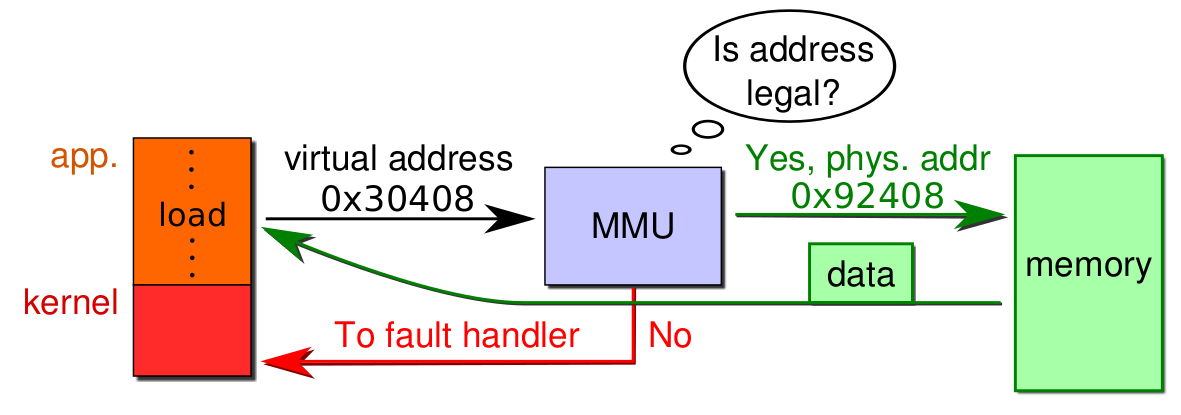
\includegraphics[width=0.33\textwidth]{MMU}\end{figure}

\paragraph{MMU --- base and limit registers}
\begin{itemize}
  \item \textbf{Idea}: provide protection + dynamic relocation in MMU
  \begin{itemize}
    \item[$ \to $] introduce special \emph{base} and \emph{limit} registers (e.g., Cray-1)
  \end{itemize}
  \item \textbf{Usage}: on every load/store the MMU 
  \begin{itemize}
    \item checks if virtual address \( \geq \) \code{base}
    \item checks if virtual address \( < \) \code{base} + \code{limit}
    \item use virtual address as physical address in memory
  \end{itemize}
  \item \textbf{Protection}: OS needs to be protected from processes
  \begin{itemize}
    \item main memory split in two partitions (low = OS, high = user processes)
    \item OS can access all process partitions (e.g., to copy syscall parameters)
    \item MMU denies processes access to OS memory
  \end{itemize}
  \item \textbf{Advantages}:
  \begin{itemize}
    \item[+] straight forward to implement MMU
    \item[+] very quick at run-time
  \end{itemize}
  \item \textbf{Disadvantages}:
  \begin{itemize}
    \item[-] how to grow process's address space?
    \item[-] how to share code/data?
  \end{itemize}
\end{itemize}
\begin{figure}[h]\centering\label{MMUBaseLimit}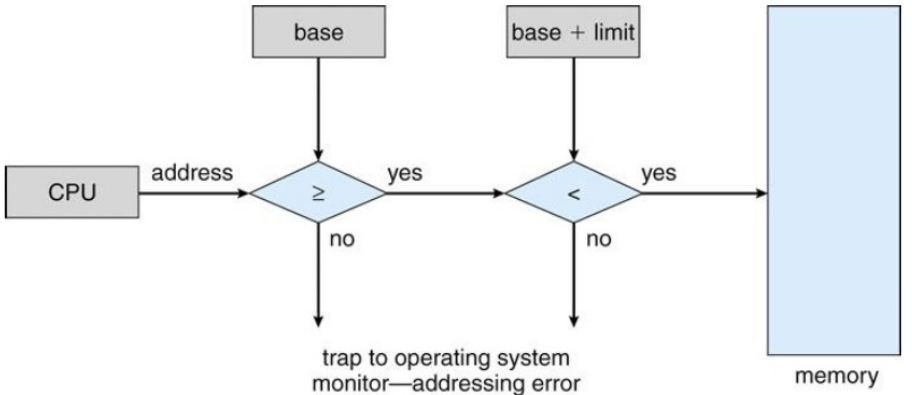
\includegraphics[width=0.33\textwidth]{MMUBaseLimit}\end{figure}

\paragraph{MMU --- Segmentation}
\begin{itemize}
  \item \textbf{Solution} to base + limit: use multiple base + limit register pairs \emph{per process}
  \begin{itemize}
    \item[$ \to $] private + public segments
  \end{itemize}
  \item \textbf{Advantages}:
  \begin{itemize}
    \item[+] data/code sharing between processes possible without compromising confidentiality
    \item[+] process does not need large contiguous physical memory area \( \to \) easy placement
    \item[+] process does not need to be entirely in memory \( \to \) memory overcommitment ok
  \end{itemize}
  \item \textbf{Disadvantages}:
  \begin{itemize}
    \item[-] segments need to be kept contiguous in physical memory
    \item[-] \emph{fragmentation} of physical memory
  \end{itemize}
\end{itemize}

\paragraph{Segmentation --- Architecture}
\begin{itemize}
  \item virtual address = [segment \#, offset]
  \item each process has \emph{segment table}, maps virtual address to physical address in memory
  \begin{itemize}
    \item \emph{base}: starting physical address where segment resides in memory
    \item \emph{limit}: length of segment
    \item \emph{protection}: access restriction (read/write) for safe sharing
  \end{itemize}
  \item MMU has two registers that identify current address space
  \begin{itemize}
    \item \emph{segment-table base register} (STBR): points to segment table location of current process
    \item \emph{segment-table length register} (STLR): indicates number of segments used by process
  \end{itemize}
\end{itemize}
\begin{figure}[h]\centering\label{Segmentation}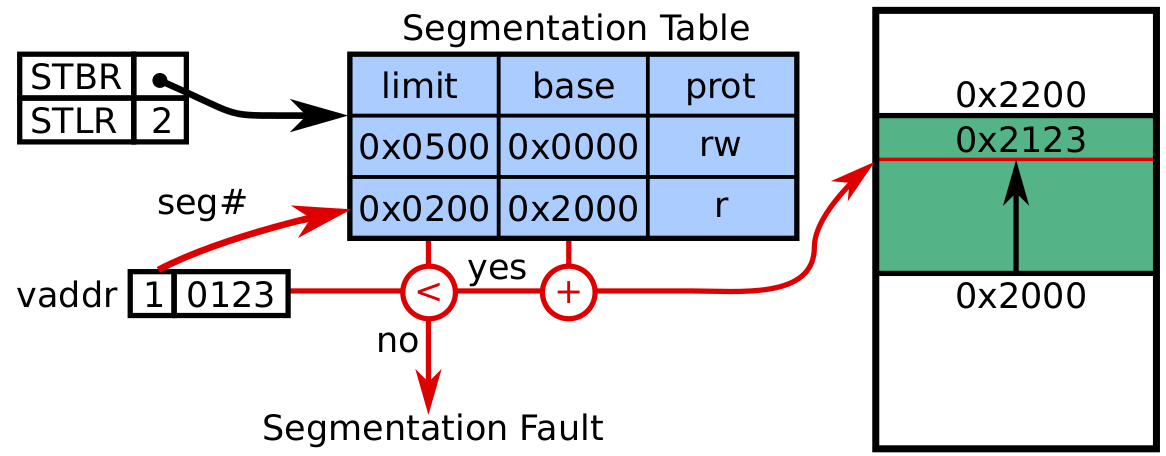
\includegraphics[width=0.33\textwidth]{Segmentation}\end{figure}

\paragraph{External Fragmentation}
\begin{itemize}
  \item \textbf{Fragmentation} = inability to use free memory
  \item \textbf{External Fragmentation} = sum of free memory satisfies requested amount of memory, but is not contiguous
  \item \textbf{Compaction}: reduce external fragmentation
  \begin{itemize}
    \item close gaps by moving allocated memory in one direction
    \item only possible if relocation is dynamic, can be done at execution time
    \item \emph{problem}: expensive! Need to halt process while moving data and updating tables
    \begin{itemize}
      \item[$ \to $] caches need to be reloaded, which should be avoided 
    \end{itemize}
  \end{itemize}
\end{itemize}

\paragraph{MMU --- Paging}
\begin{itemize}
  \item \textbf{Principle}: divide physical memory into fixed-size blocks (\emph{page frames})
  \begin{itemize}
    \item size = \( 2^n \) Bytes (typically 4KiB, 2MiB, 4MiB)
  \end{itemize}
  \item \textbf{Virtual Memory}: divided into same-sized blocks (\emph{pages})
  \item \textbf{Page Table}: managed by OS, stores mappings between \emph{virtual page numbers} (vpn) and \emph{page frame numbers} (pfn) for each AS
  \item OS tracks all free frames, modifies page tables as needed
  \item \textbf{Present Bit} (in page table): indicates that virtual page is currently mapped to physical memory
  \item if process issues instruction to access unmapped virtual address, MMU calls OS to bring in the data (\emph{page fault})
\end{itemize}

\paragraph{MMU --- Address Translation Scheme}
\begin{itemize}
  \item \textbf{Virtual address}: divided into
  \begin{itemize}
    \item \emph{virtual page number}: page table index containing base address of each page in physical memory
    \item \emph{page offset}: concatenated with base address results in physical address
  \end{itemize}
\end{itemize}

\paragraph{MMU --- Hierarchical Page Table}
\begin{itemize}
  \item \textbf{Problem}: need to keep complete page table in memory for every address space
  \item \textbf{Idea}: not needing complete table, most virtual addresses unused by process
  \begin{itemize}
    \item[$ \to $] subdivide virtual address further into multiple page indexes \( p_n \) forming \emph{hierarchical page table}
  \end{itemize}
\end{itemize}

\paragraph{Hierarchical Page Table --- x86-64}
\begin{itemize}
  \item \textbf{long mode}: 4-level hierarchical page table
  \item \textbf{page directory base register} (control register 3, \code{\%CR3}) stores starting physical address of \emph{first level page table}
  \item \textbf{address-space hierarchy}: following page-table hierarchy for every address space:
  \begin{itemize}
    \item page map level 4 (PML4)
    \item page directory pointers table (PDPT)
    \item page directory (PD)
    \item page table entry (PTE)
  \end{itemize}
  \item \textbf{Per level}: table can either point to \emph{directory} in next hierarchy level or to \emph{entry} containing actual mapping data
\end{itemize}
\begin{figure}[h]\centering\label{PageTable}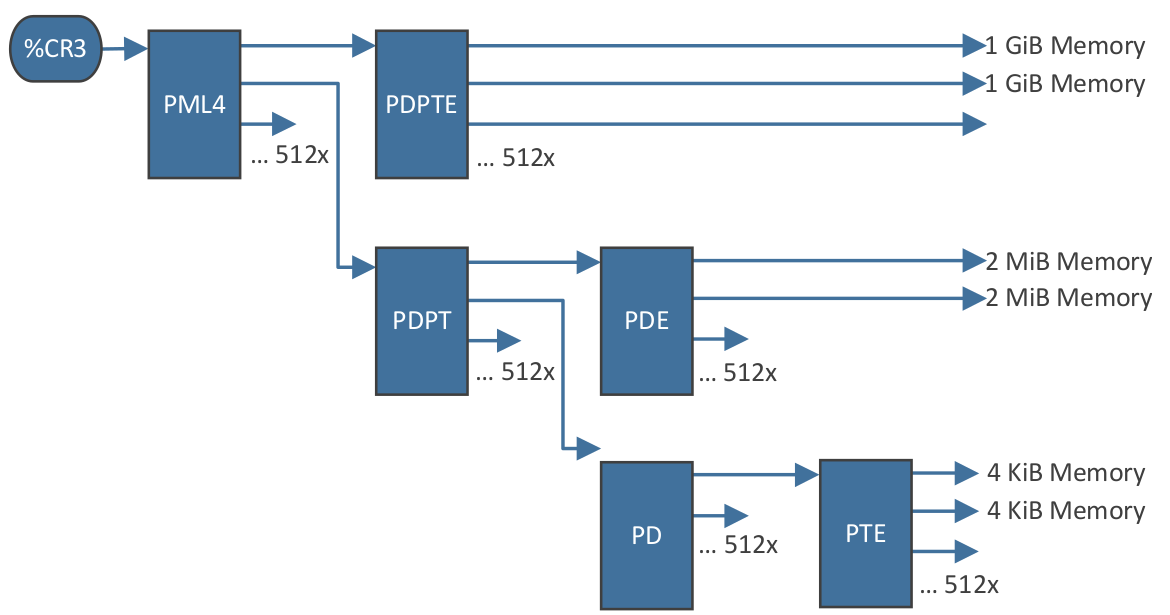
\includegraphics[width=0.33\textwidth]{PageTable}\end{figure}

\paragraph{Page Table Entry --- Content}
\begin{itemize}
  \item \textbf{valid bit} (\emph{present bit}): whether page is currently available in memory or needs to be brought in by OS via \emph{page fault}
  \item \textbf{page frame number}: if page is present: physical address where page is currently located
  \item \textbf{write bit}: whether or not page may be written to (may cause \emph{page fault})
  \item \textbf{caching}: whether or not page should be cached at all (and with which policy)
  \item \textbf{accessed bit}: set by MMU if page was touched since bit was last cleared by OS
  \item \textbf{dirty bit}: set by MMU if page was modified since bit was last cleared by OS
\end{itemize}

\paragraph{Paging --- OS Involvement}
\begin{itemize}
  \item OS performs all operations that require semantic knowledge
  \item \textbf{page allocation} (bringing data into memory): OS needs to find free frame for new pages and set up mapping in page table of affected address space
  \item \textbf{page replacement}: when all page frames are used, OS needs to evict pages from memory
  \item \textbf{context switching}: OS sets MMU's base register (\code{\%CR3} on x86) to point to page hierarchy of next process's address space
\end{itemize}

\paragraph{MMU --- Internal Fragmentation}
\begin{itemize}
  \item \textbf{Paging}: eliminates external fragmentation
  \item \textbf{Problem}: internal fragmentation
  \begin{itemize}
    \item memory can only be allocated in page frame sizes
    \item allocated virtual memory area will generally not end at page boundary
    \item[$ \leadsto $] unused rest of last allocated page is lost!
  \end{itemize}
\end{itemize}

\paragraph{MMU --- Page Size trade-offs}
\begin{itemize}
  \item \textbf{Fragmentation}:
  \begin{itemize}
    \item \emph{larger pages} \( \to \) more memory wasted (internal fragmentation) per allocation
    \item \emph{smaller pages} \( \to \) only half a page wasted per allocation on average
  \end{itemize}
  \item \textbf{Table Size}:
  \begin{itemize}
    \item \emph{larger pages} \( \to \) fewer bits needed for \code{pfn} (more bits in offset), fewer PTEs
    \item \emph{smaller pages} $ \to $ more + larger PTEs
  \end{itemize}
  \item \textbf{I/O}:
  \begin{itemize}
    \item \emph{larger pages} $ \to $ more data needs to be loaded from dist to make page valid
    \item \emph{smaller pages} $ \to $ need to trap OS more often when loading large program
  \end{itemize}
\end{itemize}

\begin{summary}
  \begin{itemize}
    \item need to place processes in memory to run
    \item want to place multiple processes in memory at same time to run concurrently/parallel
    \item \textbf{Virtual Memory}: enables protection, transparency, overcommitment
    \begin{itemize}
      \item \emph{trade-off} extra hardware (MMU) to translate addresses at every load/store
    \end{itemize}
    \item \textbf{MMU types}: base + limit, segmentation, paging
    \item \textbf{Paging}: supported by all contemporary MMUs, favored by most OS
  \end{itemize}
\end{summary}
